\documentclass[17pt, a1paper, portrait, margin=12mm, innermargin=13mm,
               blockverticalspace=5mm, colspace=11mm, subcolspace=6mm]{tikzposter}

\usepackage[utf8]{inputenc}
\usepackage[T1]{fontenc}
\usepackage{mathptmx}
\usepackage{graphicx}
\usepackage{amsmath,amssymb}
\usepackage{enumitem}
\usepackage{ragged2e}
\usepackage{tikz}
\usetikzlibrary{shapes.geometric, arrows.meta, positioning}
\setlist[itemize]{leftmargin=*,itemsep=3pt,topsep=3pt,parsep=0pt,label=\textcolor{accent}{$\blacktriangleright$}}
\hyphenpenalty=10000
\exhyphenpenalty=10000
\emergencystretch=1em

% ---------- colours ----------
\definecolor{charcoal}{RGB}{58,58,58}
\definecolor{lightblue}{RGB}{219,230,244}
\definecolor{navy}{RGB}{20,52,110}
\definecolor{accent}{RGB}{14,110,120}
\definecolor{orange}{RGB}{200,110,30}
\definecolor{leaf}{RGB}{76,140,74}

\definecolorstyle{codeec}{}{
  \colorlet{titlefgcolor}{black}
  \colorlet{backgroundcolor}{white}
  \colorlet{blocktitlebgcolor}{lightblue}
  \colorlet{blocktitlefgcolor}{navy}
  \colorlet{blockbodybgcolor}{lightblue}
  \colorlet{blockbodyfgcolor}{black}
  \colorlet{innerblocktitlebgcolor}{white}
  \colorlet{innerblocktitlefgcolor}{navy}
  \colorlet{notebgcolor}{white}
  \colorlet{notefrcolor}{navy}
  \colorlet{notefgcolor}{black}
  \colorlet{framecolor}{navy}
}
\usecolorstyle{codeec}
\usebackgroundstyle{Empty}
\usetitlestyle{Empty}
\useblockstyle{Default}
\tikzposterlatexaffectionproofoff

% ---------- icon helper (small inline tikz) ----------
\newcommand{\icon}[1]{\,\raisebox{-1mm}{\begin{tikzpicture}[scale=0.9]#1\end{tikzpicture}}\,}
% individual icons
\newcommand{\icProblem}{\icon{\draw[line width=1.4pt,accent] (0,0) circle (0.42); \node[accent,font=\bfseries] at (0,0) {?};}}
\newcommand{\icGoal}{\icon{\draw[line width=1.4pt,accent] (0,0) circle (0.42);\draw[line width=1.4pt,accent](0,0)circle(0.22);\fill[accent](0,0)circle(0.06);}}
\newcommand{\icGap}{\icon{\draw[line width=1.4pt,accent](-0.4,0.3)--(0.4,0.3);\draw[line width=1.4pt,accent,dashed](-0.4,-0.1)--(0.4,-0.1);\draw[line width=1.4pt,accent](-0.4,-0.4)--(0.0,-0.4);}}
\newcommand{\icFramework}{\icon{\draw[line width=1.3pt,accent,fill=accent!15](-0.4,0.15)rectangle(0.4,0.45);\draw[line width=1.3pt,accent,fill=accent!15](-0.4,-0.45)rectangle(0.4,-0.15);\draw[->,line width=1.2pt,accent](0,0.15)--(0,-0.15);}}
\newcommand{\icObjectives}{\icon{\draw[line width=1.4pt,accent](0,-0.4)--(0,0.45);\draw[line width=1.3pt,accent,fill=orange!70](0,0.45)--(0.45,0.32)--(0,0.18)--cycle;}}
\newcommand{\icMethod}{\icon{\draw[line width=1.4pt,accent](-0.3,-0.4)--(-0.05,0.1)--(-0.05,0.45)--(0.05,0.45)--(0.05,0.1)--(0.3,-0.4)--cycle;\fill[accent!30](-0.18,-0.25)--(-0.05,0.05)--(0.05,0.05)--(0.18,-0.25)--cycle;}}
\newcommand{\icResults}{\icon{\draw[line width=1.2pt,accent](-0.45,-0.4)--(0.45,-0.4);\fill[gray!50](-0.35,-0.4)rectangle(-0.15,0.0);\fill[accent](0.05,-0.4)rectangle(0.25,0.35);}}
\newcommand{\icContrib}{\icon{\draw[line width=1.3pt,accent,fill=orange!60](0,0.45)--(0.13,0.13)--(0.45,0.13)--(0.2,-0.08)--(0.28,-0.4)--(0,-0.2)--(-0.28,-0.4)--(-0.2,-0.08)--(-0.45,0.13)--(-0.13,0.13)--cycle;}}
\newcommand{\icPlan}{\icon{\draw[line width=1.3pt,accent](-0.45,0.35)rectangle(0.45,-0.45);\draw[line width=1pt,accent](-0.45,0.15)--(0.45,0.15);\fill[accent!60](-0.35,-0.05)rectangle(0.05,0.05);\fill[accent!60](-0.2,-0.25)rectangle(0.3,-0.15);}}
\newcommand{\icRef}{\icon{\draw[line width=1.3pt,accent](-0.3,-0.45)--(-0.3,0.45)--(0.3,0.45)--(0.3,-0.45)--cycle;\draw[line width=1pt,accent](-0.15,0.25)--(0.15,0.25);\draw[line width=1pt,accent](-0.15,0.05)--(0.15,0.05);\draw[line width=1pt,accent](-0.15,-0.15)--(0.15,-0.15);}}

% ---------- custom title / header ----------
\settitle{
\begin{minipage}{\linewidth}
  \setlength{\fboxsep}{10pt}%
  \colorbox{charcoal}{\makebox[\dimexpr\linewidth-2\fboxsep\relax][l]{%
    \color{white}%
    \begin{minipage}[c][2.1cm][c]{0.45\linewidth}%
      {\fontsize{42}{46}\selectfont\textbf{CoDEEC 2026}}\\[3pt]
      {\large Summer Edition \textemdash\ 17 June 2026}
    \end{minipage}\hfill
    \raisebox{-0.5\height}{
\includegraphics[height=1.8cm]{uc_white.png}}\hfill
    \raisebox{-0.5\height}{
\includegraphics[height=1.15cm]{deec.png}}%
  }}\\[0.45cm]
  \begin{minipage}[c]{0.80\linewidth}\RaggedRight
    \resizebox{\linewidth}{!}{\bfseries\color{navy}Reliable Multi-Scale Sensor Fusion Framework for Agricultural Robots}\\[0.4cm]
    {\fontsize{28}{32}\selectfont\textbf{Syed Bukhari}}\\[0.25cm]
    {\large Supervisor: Prof.\ Gil Gon\c{c}alves \quad\textbar\quad Co-supervisor: Prof.\ Lino Jos\'e Forte Marques}\\[2pt]
    {\large PhD in Electrical Engineering and Intelligent Systems, University of Coimbra}
  \end{minipage}\hfill
  \begin{minipage}[c]{0.18\linewidth}\raggedleft
    
\includegraphics[width=1.0\linewidth]{isr.png}
  \end{minipage}
\end{minipage}
}

\begin{document}
\maketitle[width=\textwidth, titletoblockverticalspace=5mm]

% ===== ROW 1: Problem | Goal | SOTA =====
\begin{columns}
\column{0.34}
\block{\icProblem\ Problem}{\RaggedRight
\textbf{Robots need crop \& field state} across many scales --- one plant to a whole region.
\begin{center}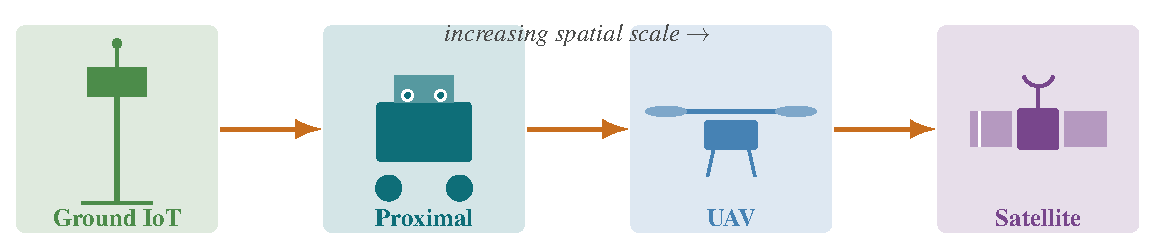
\includegraphics[width=0.98\linewidth]{scales_viz.pdf}\end{center}
\begin{itemize}
  \item No single sensor sees all scales.
  \item Demands principled \textbf{multi-scale fusion}.
\end{itemize}
}
\column{0.32}
\block{\icGoal\ Goal}{\RaggedRight
A \textbf{reliable multi-scale fusion framework}:
\begin{itemize}
  \item Fuse \textbf{ground IoT $\cdot$ proximal $\cdot$ UAV $\cdot$ satellite}.
  \item \textbf{Calibrated uncertainty} + dynamic \textbf{digital twin}.
  \item Validated \textbf{in the field}.
\end{itemize}
}
\column{0.34}
\block{\icGap\ State of the Art \& Gap}{\RaggedRight
Fusion is mature (Bayesian/Kalman $\to$ deep learning) [1]; agri remote-sensing fusion [2] \& digital twins [3] are growing.
\begin{itemize}
  \item Mostly \textbf{single-scale}, \textbf{offline}.
  \item Reliability under \textbf{degraded data} ignored.
  \item Perception$\to$twin$\to$robot loop unexplored.
\end{itemize}
}
\end{columns}

% ===== ROW 2: Framework (big viz) | Objectives =====
\begin{columns}
\column{0.66}
\block{\icFramework\ Proposed Framework}{
\begin{center}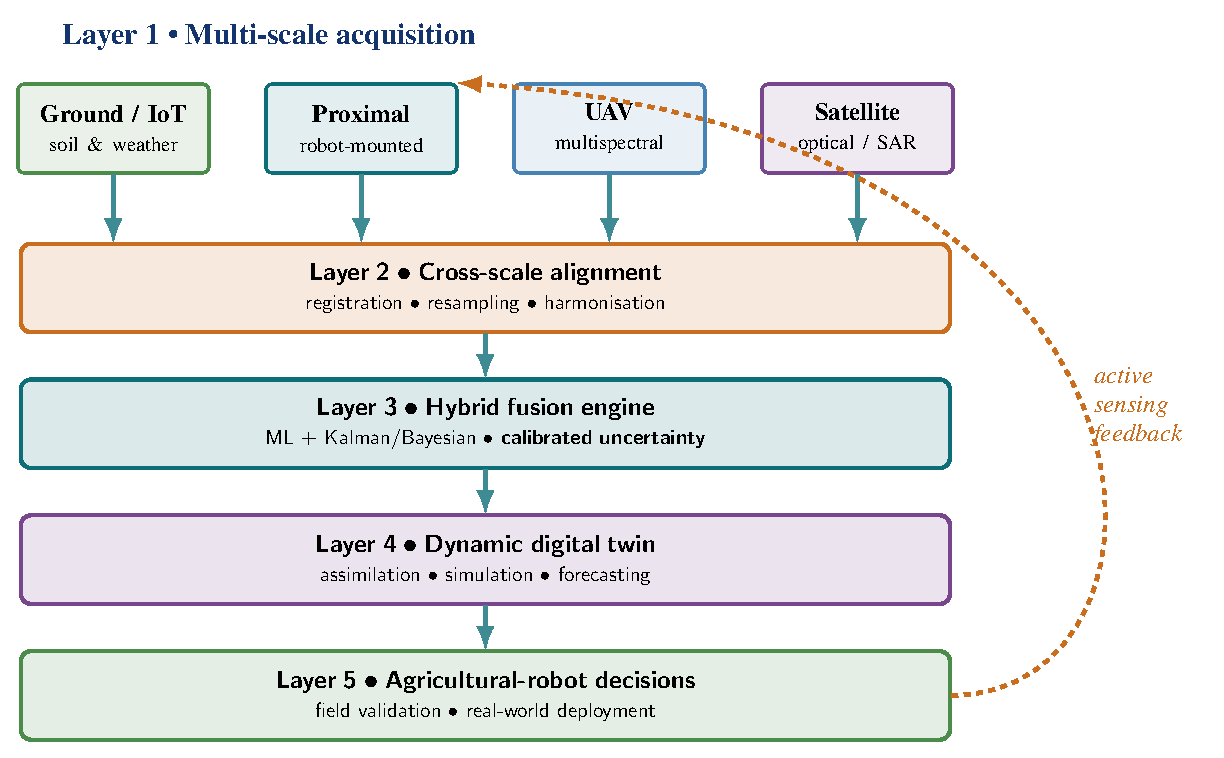
\includegraphics[width=0.74\linewidth]{framework_viz.pdf}\end{center}
}
\column{0.34}
\block{\icObjectives\ Objectives}{\RaggedRight
\begin{itemize}
  \item[\textcolor{orange}{\textbf{O1}}] Systematic review.
  \item[\textcolor{orange}{\textbf{O2}}] IoT pipeline \& alignment.
  \item[\textcolor{orange}{\textbf{O3}}] Baseline fusion prototypes.
  \item[\textcolor{orange}{\textbf{O4}}] Uncertainty-aware engine.
  \item[\textcolor{orange}{\textbf{O5}}] Couple to digital twin.
  \item[\textcolor{orange}{\textbf{O6}}] Field \& robot validation.
\end{itemize}
}
\end{columns}

% ===== ROW 3: Methodology | Results (chart) | Contributions =====
\begin{columns}
\column{0.34}
\block{\icMethod\ Methodology}{\RaggedRight
\begin{itemize}
  \item \textbf{Align:} registration \& harmonisation.
  \item \textbf{Fuse:} ML + Kalman/Bayesian.
  \item \textbf{Reliability:} calibrated, robust to dropout.
  \item \textbf{Twin:} simulate \& forecast.
  \item \textbf{Validate:} accuracy \& robustness.
\end{itemize}
\vspace{1mm}
{\centering\large\textbf{Pilot study area}\par}
\begin{center}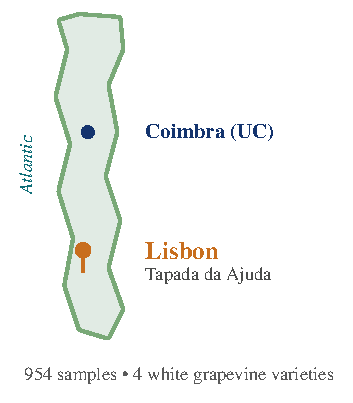
\includegraphics[width=0.38\linewidth]{map_viz.pdf}\end{center}
}
\column{0.32}
\block{\icResults\ Preliminary Results}{
\begin{center}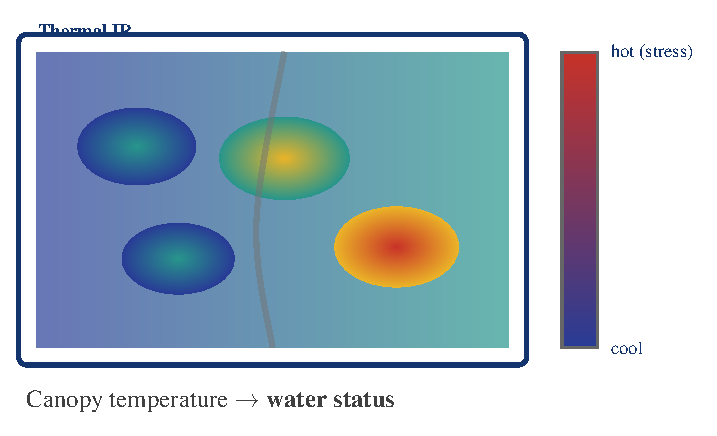
\includegraphics[width=0.54\linewidth]{thermal_viz.pdf}\end{center}
\vspace{1mm}
\begin{center}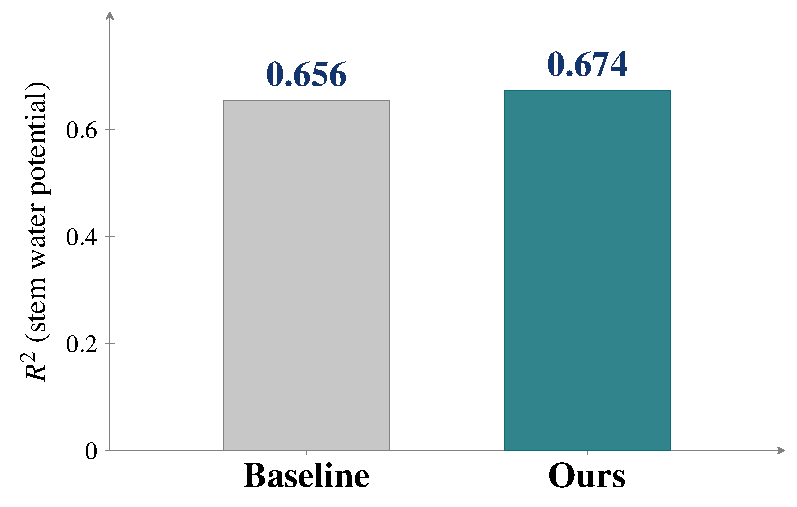
\includegraphics[width=0.50\linewidth]{results_chart.pdf}\end{center}
\vspace{0.5mm}
{\centering\large Ground-scale \textbf{thermal pilot}: \textbf{$>$87\%} wins $\cdot$ skewness \textbf{$\downarrow$26--55\%} $\cdot$ variety-agnostic.\par}
}
\column{0.34}
\block{\icContrib\ Expected Contributions}{\RaggedRight
\begin{itemize}
  \item Uncertainty-aware fusion framework.
  \item IoT pipeline \& aligned dataset.
  \item Hybrid ML + probabilistic fusion.
  \item Digital twin $+$ active sensing.
  \item Real-world robot validation.
\end{itemize}
}
\end{columns}

% ===== ROW 4: Work Plan (gantt) | References =====
\begin{columns}
\column{0.66}
\block{\icPlan\ Work Plan (48 months)}{
\begin{center}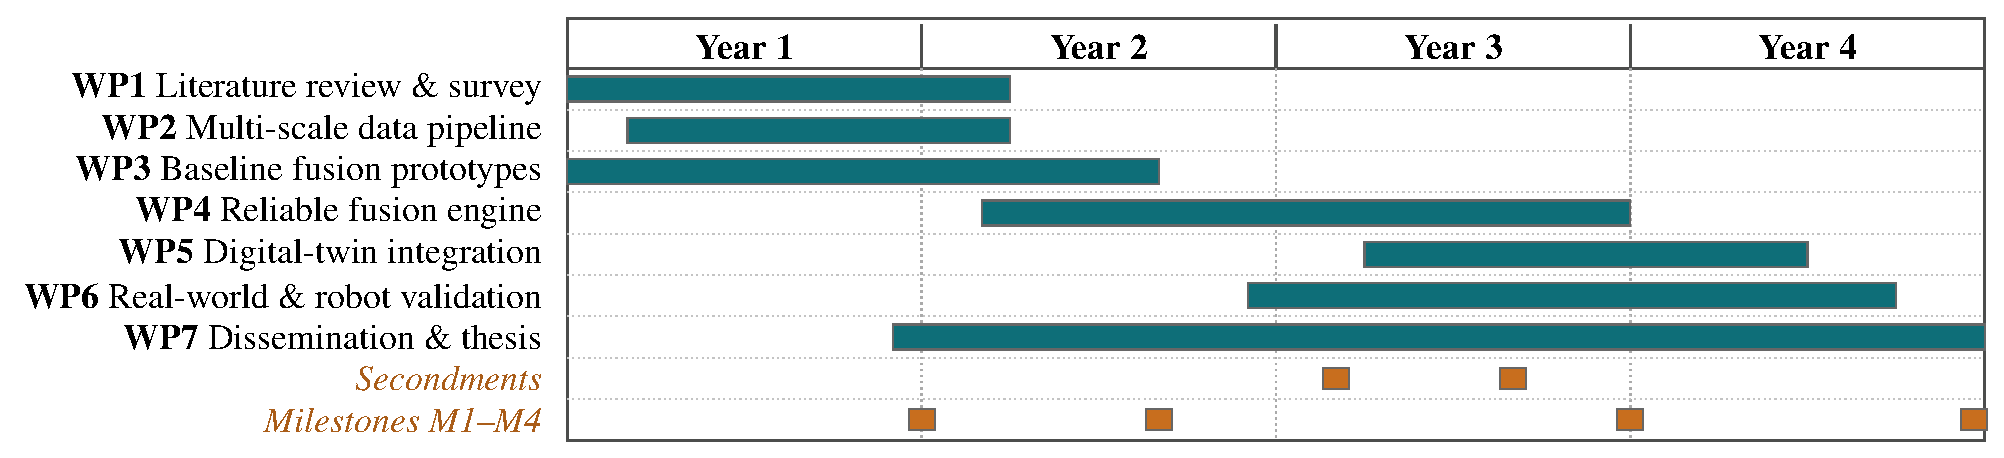
\includegraphics[width=0.87\linewidth]{gantt_viz.pdf}\end{center}
}
\column{0.34}
\block{\icRef\ References}{\RaggedRight
\small
{[1]} Khaleghi \textit{et al.}, \textit{Information Fusion}, 2013.\\
{[2]} Ghamisi \textit{et al.}, \textit{IEEE GRSM}, 2019.\\
{[3]} Peladarinos \textit{et al.}, \textit{Sensors}, 2023.\\
{[4]} Pires \textit{et al.}, \textit{Comput.\ Electron.\ Agric.}, 2025.
}
\end{columns}

% ===== FULL-WIDTH ACKNOWLEDGMENT BOX =====
\block{}{\centering\large
This work is carried out within the \textbf{AIGreenBots} project, funded by the European Union under MSCA Grant Agreement No.~101169330, with the support of \textbf{ISR-UC}, \textbf{INESC Coimbra}, and the \textbf{University of Coimbra}.\par}

\end{document}
